\documentclass{beamer}[10pt, usepdftitle=false, handout]

\beamertemplatenavigationsymbolsempty

\usepackage[T1]{fontenc}
\usepackage[]{algorithm2e}
\usepackage{multimedia}
\usepackage{gensymb}
\usepackage{textcomp}
%\usepackage{background}
%\backgroundsetup{
%    placement=center,
%    scale=1,
%    contents={The author of this course is PAUL BLONDEL},
%    opacity=0.7
%}
%\setbeamertemplate{background}{\BgMaterial}

%\usepackage[font=small,labelfont=bf]{caption} 

\usetheme{Boadilla}

\title{Operating system principles 2}
\author[]{Paul Blondel}
\institute[]{CNAM}
\date[]{September 1st, 2018}

\usepackage[style=british]{csquotes}


\def\signed #1{{\leavevmode\unskip\nobreak\hfil\penalty50\hskip1em
  \hbox{}\nobreak\hfill #1%
  \parfillskip=0pt \finalhyphendemerits=0 \endgraf}}

\newsavebox\mybox
\newenvironment{aquote}[1]
  {\savebox\mybox{#1}\begin{quote}\openautoquote\hspace*{-.7ex}}
  {\unskip\closeautoquote\vspace*{1mm}\signed{\usebox\mybox}\end{quote}}


%\setbeamertemplate{headline}
%{
%  \leavevmode%
%  \hbox{%
%  \begin{beamercolorbox}[wd=1.0\paperwidth,ht=2.25ex,dp=1ex,center]{author in head/foot}%
%    \textcolor{green}{- This course has been made by Paul Blondel -} \usebeamerfont{author in head/foot}\insertsubsection
%  \end{beamercolorbox}}%
%  \vskip0pt%
%}


\setbeamertemplate{footline}
{
  \leavevmode%
  \hbox{%
  \begin{beamercolorbox}[wd=.5\paperwidth,ht=2.25ex,dp=1ex,center]{author in head/foot}%
    \usebeamerfont{author in head/foot}\insertsection
  \end{beamercolorbox}%
  \begin{beamercolorbox}[wd=.5\paperwidth,ht=2.25ex,dp=1ex,center]{title in head/foot}%
    \usebeamerfont{title in head/foot} \inserttitle \hspace*{2em}  \insertframenumber{} / \inserttotalframenumber\hspace*{2ex} 
  \end{beamercolorbox}}%
  \vskip0pt%
}

\AtBeginSection[]
{
   \begin{frame}
    \tableofcontents[ 
    currentsection,
    hideallsubsections] 
   \end{frame}
}

\begin{document}
	{
	\setbeamertemplate{footline}{
  	\leavevmode%
  	\hbox{%
  	\begin{beamercolorbox}[wd=.5\paperwidth,ht=2.25ex,dp=1ex,center]{author in head/foot}%
  	\end{beamercolorbox}%
  	\begin{beamercolorbox}[wd=.5\paperwidth,ht=2.25ex,dp=1ex,center]{title in head/foot}%
  	\end{beamercolorbox}}%
  	\vskip0pt%	
	} 
	\begin{frame}
	\titlepage
	\end{frame}

	\begin{frame}
	
	\begin{aquote}{Eric S. Raymond}
	(Kenneth) Thompson and (Dennis) Ritchie were among the first to realize that hardware and compiler technology had become good enough that an entire operating system could be written in C, and by 1978 the whole environment had been successfully ported to several machines of different types.	
	\end{aquote}	
	
	\end{frame}

	\begin{frame}
		\tableofcontents[hideallsubsections]
	\end{frame}
	}

	\addtocounter{framenumber}{-3}

	\section{Processes}
	\subsection{Recall}	

    \begin{frame}[label=(first)]
	
	Recall about the \textit{compiler} and the \textit{link editor}:
	
	\vspace*{1em}	
	
	\begin{itemize}
	\item{The executable is produced by the \textit{compiler} and the \textit{link editor}}
	\item{The \textit{loader} loads it into the \textit{main memory}}
	\item{When the executable start being \textit{executed}:
		\vspace*{0.5em}
		\begin{enumerate}
			\item{The first instruction is set in the \textit{RI} register}
			\item{The address of the next instruction is set in the \textit{CO} register}
			\item{When executed: new instruction is set in \textit{RI}}
			\item{It's new next instruction address is set in \textit{CO}}
			\item{etc}
		\end{enumerate}			
	
	}	
	\end{itemize}		
	
	
    \end{frame}
    
	\subsection{Introduction}    
    
	\begin{frame}
	
	\begin{block}{So what is a process?}
	A process is an instance of an executable, it represents:
	\begin{itemize}
	\item{the state of the executable \textbf{in the processor unit}}
	\item{the state of the executable \textbf{in the main memory}}
	\end{itemize}
	\end{block}	
	
	\vspace*{1em}	
	
	Let's represent a \textit{process} as follows:
	
	\vspace*{1em}
		
	\begin{center}
		
	\begin{figure}
		
\includegraphics[scale=0.15]{images/process.png} 
     	%\vspace*{-0.5em}
		%\caption{Floating gate transistor cell}
	\end{figure}
	
	\end{center}		
	
	\end{frame}	
	
	\begin{frame}
	
	A process can be in one of these three different \textbf{states}:
	\vspace*{1em}
	\begin{enumerate}
	\item{\textbf{elected}: the process is \textbf{executed by the processor}}
	\item{\textbf{blocked}: the process is \textbf{waiting for a resource or another process}}
	\item{\textbf{ready}: the process \textbf{can be elected}, but the processor is busy}
	\end{enumerate}

	\vspace*{1em}

	\pause

	When a process goes...
	\vspace*{1em}
	\begin{itemize}
	\item{...from \textit{ready state} to \textit{elected state}: \textbf{election operation}}
	\item{...from \textit{elected state} to \textit{blocked state}: \textbf{blocking operation}}
	\item{...from \textit{blocked state} to \textit{ready state}: \textbf{unblocking operation}}
	\end{itemize}		
		
	\end{frame}

	\begin{frame}

	\begin{block}{Processes}
	Are always created in \textit{ready} state and always finishes in \textit{elected} state\footnotemark[1]
	\end{block}	
	
	\vspace*{1em}  
	
	\begin{center}
		
	\begin{figure}
		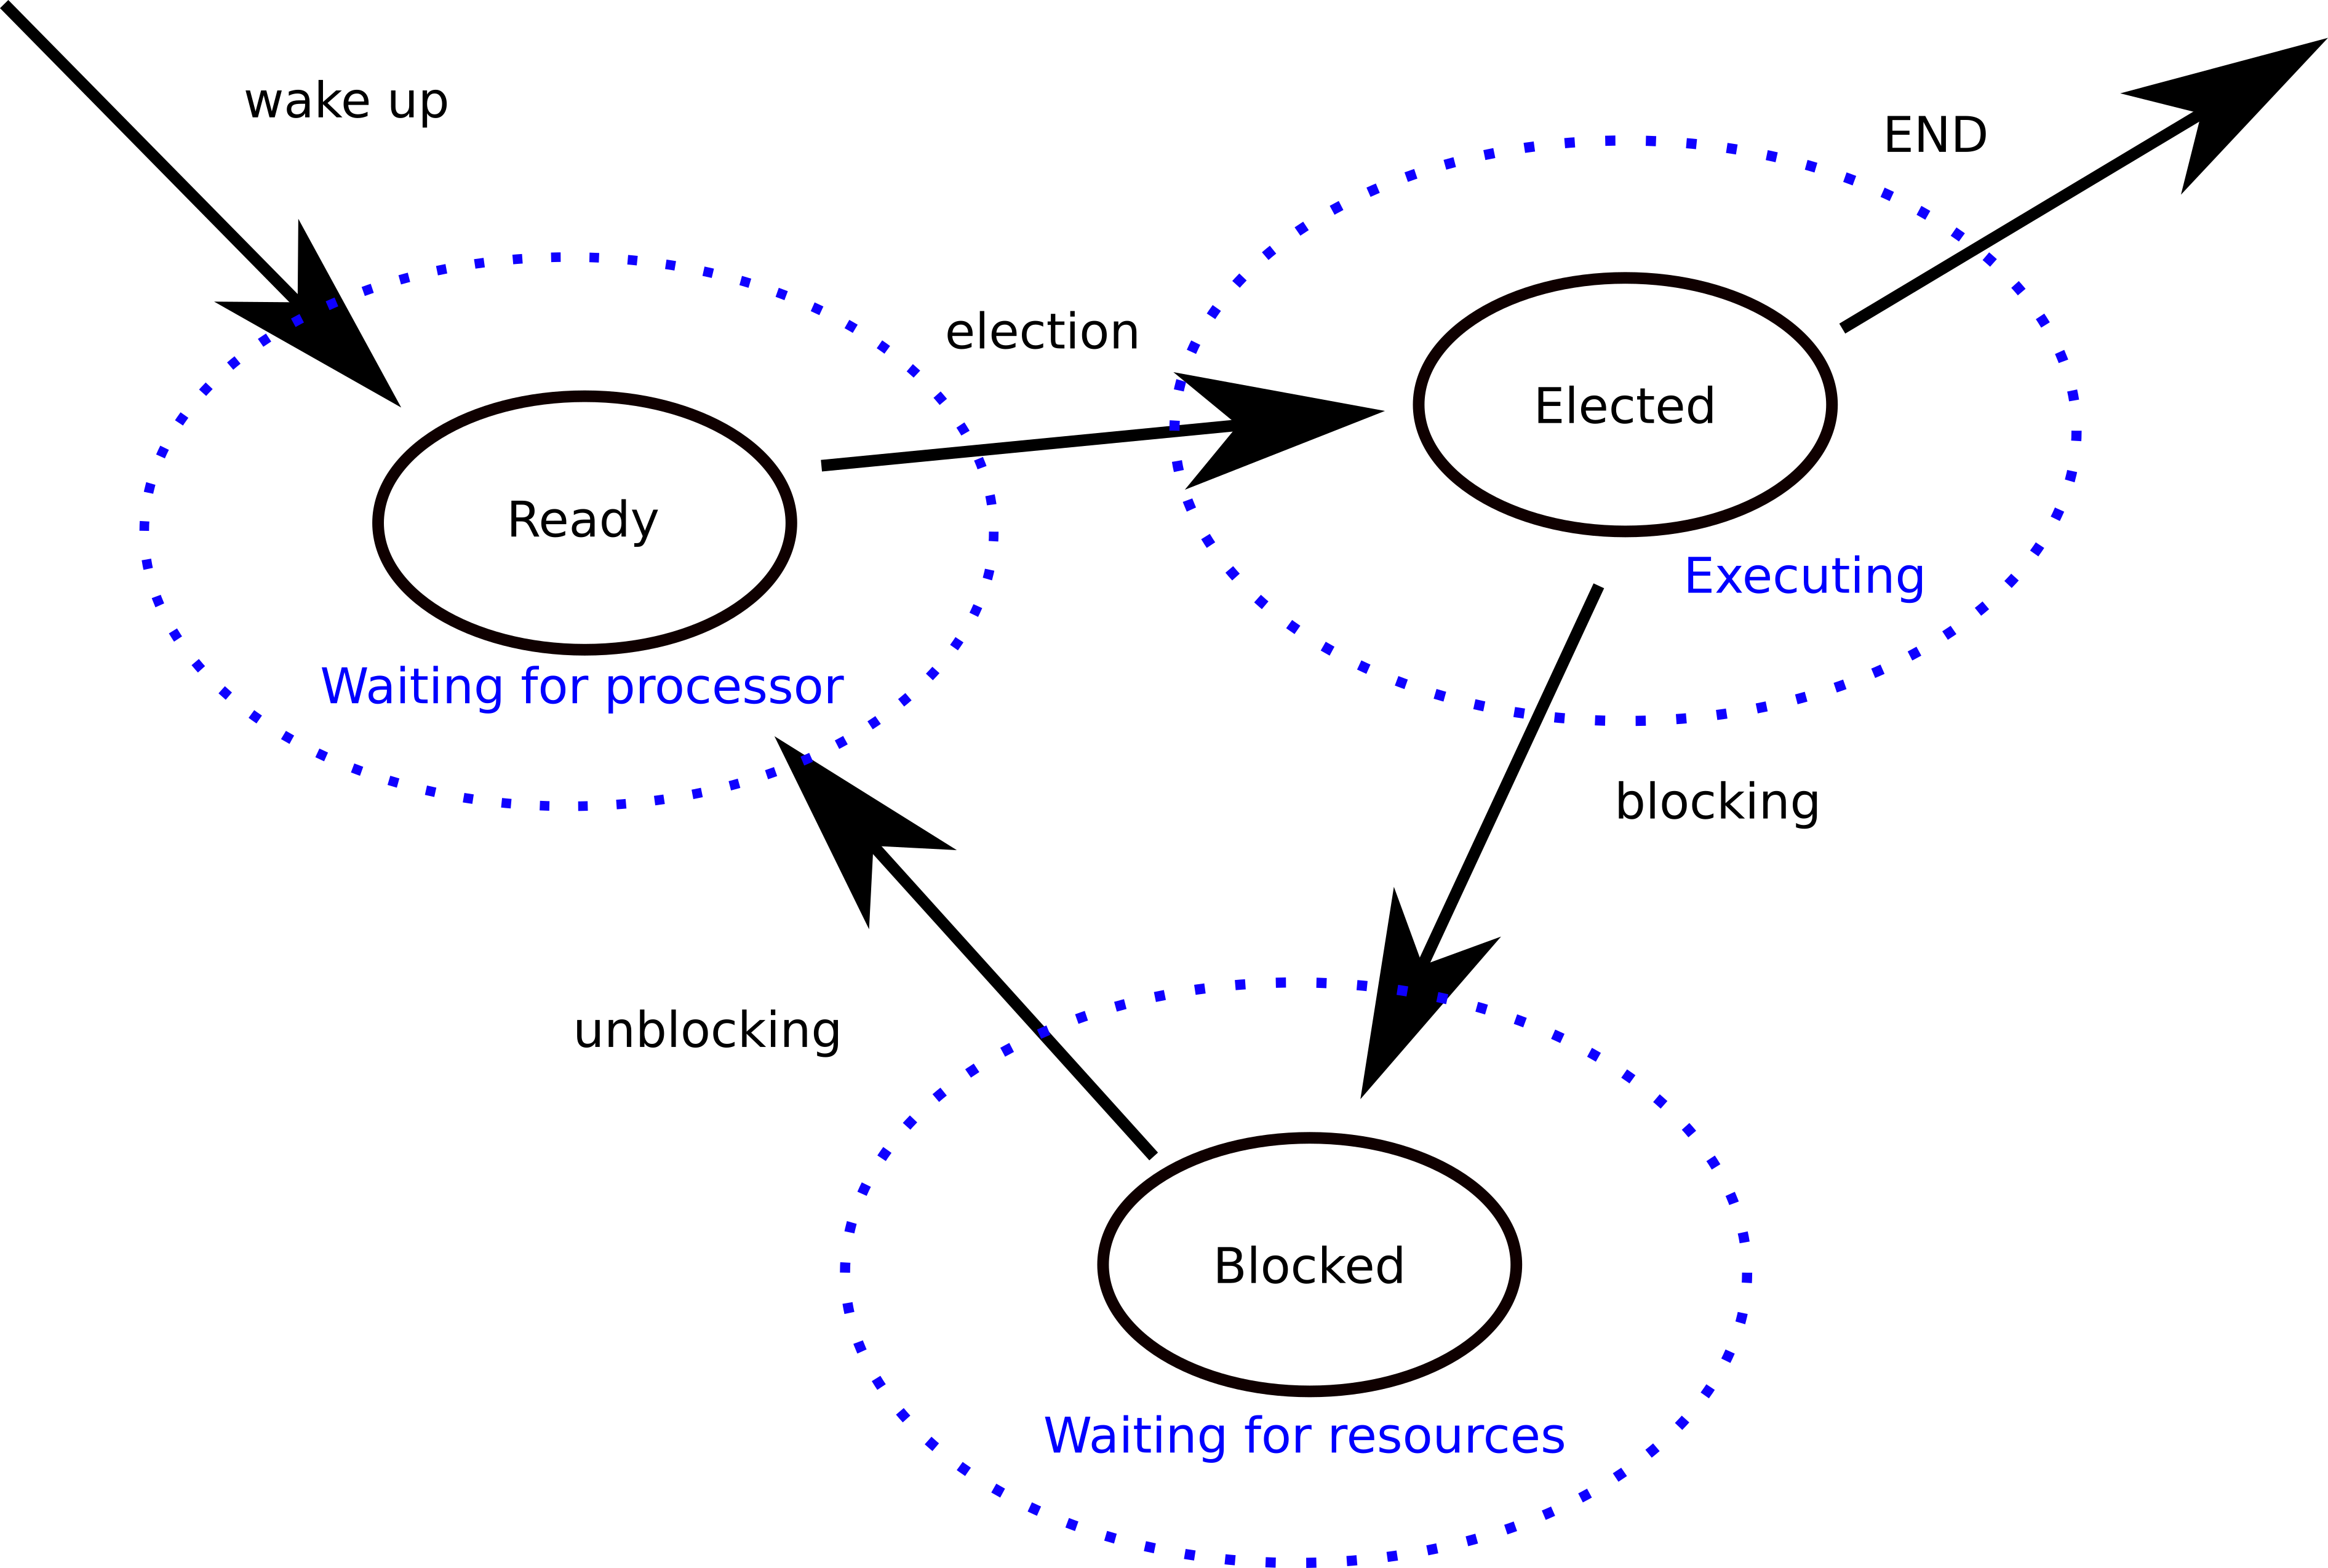
\includegraphics[scale=0.15]{images/states.png} 
     	%\vspace*{-0.5em}
		%\caption{Floating gate transistor cell}
	\end{figure}
	
	\end{center}		
	

	\footnotetext[1]{Except in case of anomalies}
	
	\end{frame}
	
	\subsection{Process Control Block}	
		
	\begin{frame}
	
	When \textit{launching} an executable:
	\vspace*{1em}
	\begin{enumerate}
	\item{The \textit{loader} \textbf{loads in \textit{main memory} the executable}}
	\item{And \textbf{create a \textit{Process Control Block} (or \textit{PCB})}}
	\end{enumerate}
		
	\pause
	\vspace*{1em}
	A \textit{PCB} contains the following information:
	\vspace*{1em}		
	\begin{itemize}
	\item{a \textbf{unique process identifier}}
	\item{a \textbf{processor context or state} (value of CO/RI, etc)}
	\item{a \textbf{memory context or state}:
		\begin{itemize}
		\item{where to get the executable instructions}
		\item{where to get the associated data}
		\end{itemize}
	}
	\item{\textbf{statistics}}
	\item{\textbf{scheduling information}}
	\item{\textbf{resource information}}
	\end{itemize}			
	
		
	\end{frame}
	
	\subsection{Creating processes}	
	
	\begin{frame}
	
	A \textit{process} can create one or more processes\footnotemark[2]:
	\vspace*{1em}
	\begin{itemize}
	\item{The creating process is called the \textbf{father process}}
	\item{Created processes are called \textbf{child processes}}
	\end{itemize}		
	
	\vspace*{1em}
	
	Depending on the system, a child \textit{process}:
	
	\begin{itemize}
	\item{may \textbf{inherit from source data and context} of the creator}
	\item{can execute a \textbf{totally different program} (Dec Vms system)}
	\item{can execute a \textbf{clone} (same data and code) (UNIX systems)}
	\end{itemize}		
	
	\begin{block}{Note}
	In some systems the father waits for the children to end to resume 
	\end{block}	
	
	\footnotetext[2]{Child processes can also create processes and become fathers, etc.}	
	
	\end{frame}	
	
	\subsection{Destructing a process}
	
	\begin{frame}
	
	The \textit{destruction} of a \textit{process} happens when:
	\vspace*{1em}
	\begin{itemize}
	\item{The \textit{process} has \textbf{terminated its execution}
		\begin{itemize}
		\item{It calls the \textit{exit()} function on UNIX}
		\end{itemize}
	}
	\item{The \textit{process} \textbf{gets an unsolvable error}}
	\item{Another \textit{process} asks the \textbf{\textit{destruction} of the \textit{process}}
		\begin{itemize}
		\item{Example: the \textit{kill} command on UNIX}
		\end{itemize}			
	}
	\end{itemize}		
	\pause
	\vspace*{1em}
	
	\begin{block}{What happens during the \textit{destruction}?}	
	\begin{itemize}
		\item{The \textbf{\textit{main memory} context is destroyed} (release memory, etc)}
		\item{\textbf{\textit{Resources} are freed} and can be used by other processes}
		\item{The \textbf{\textit{PCB} is destroyed}}
	\end{itemize}
	\end{block}
	\end{frame}	
	
	\subsection{Suspending a process}	
	
	\begin{frame}
	
	\begin{block}{What is suspending a process?}
	It is \textbf{momentarily stop the execution of a process} to resume later
	\end{block}	
	
	\vspace*{1em}	
	
	\begin{block}{What happen during the suspension?}	
	\begin{itemize}
	\item{\textit{Processor} and \textit{memory} contexts are stored in \textit{PCB}}
	\item{The state of the \textit{process} becomes \textit{blocked}}
	\end{itemize}
	\end{block}	
	
	\end{frame}	
	
	\subsection{Focus on UNIX processes}
	
	\begin{frame}
	
	\begin{block}{Note}
	UNIX systems are entirely built around the notion of \textit{processes}
	\end{block}	
	\vspace*{1em}	
	When running a UNIX system there is the following \textit{process} dependencies:
	\vspace*{1em}
	
	\begin{center}
		
	\begin{figure}
		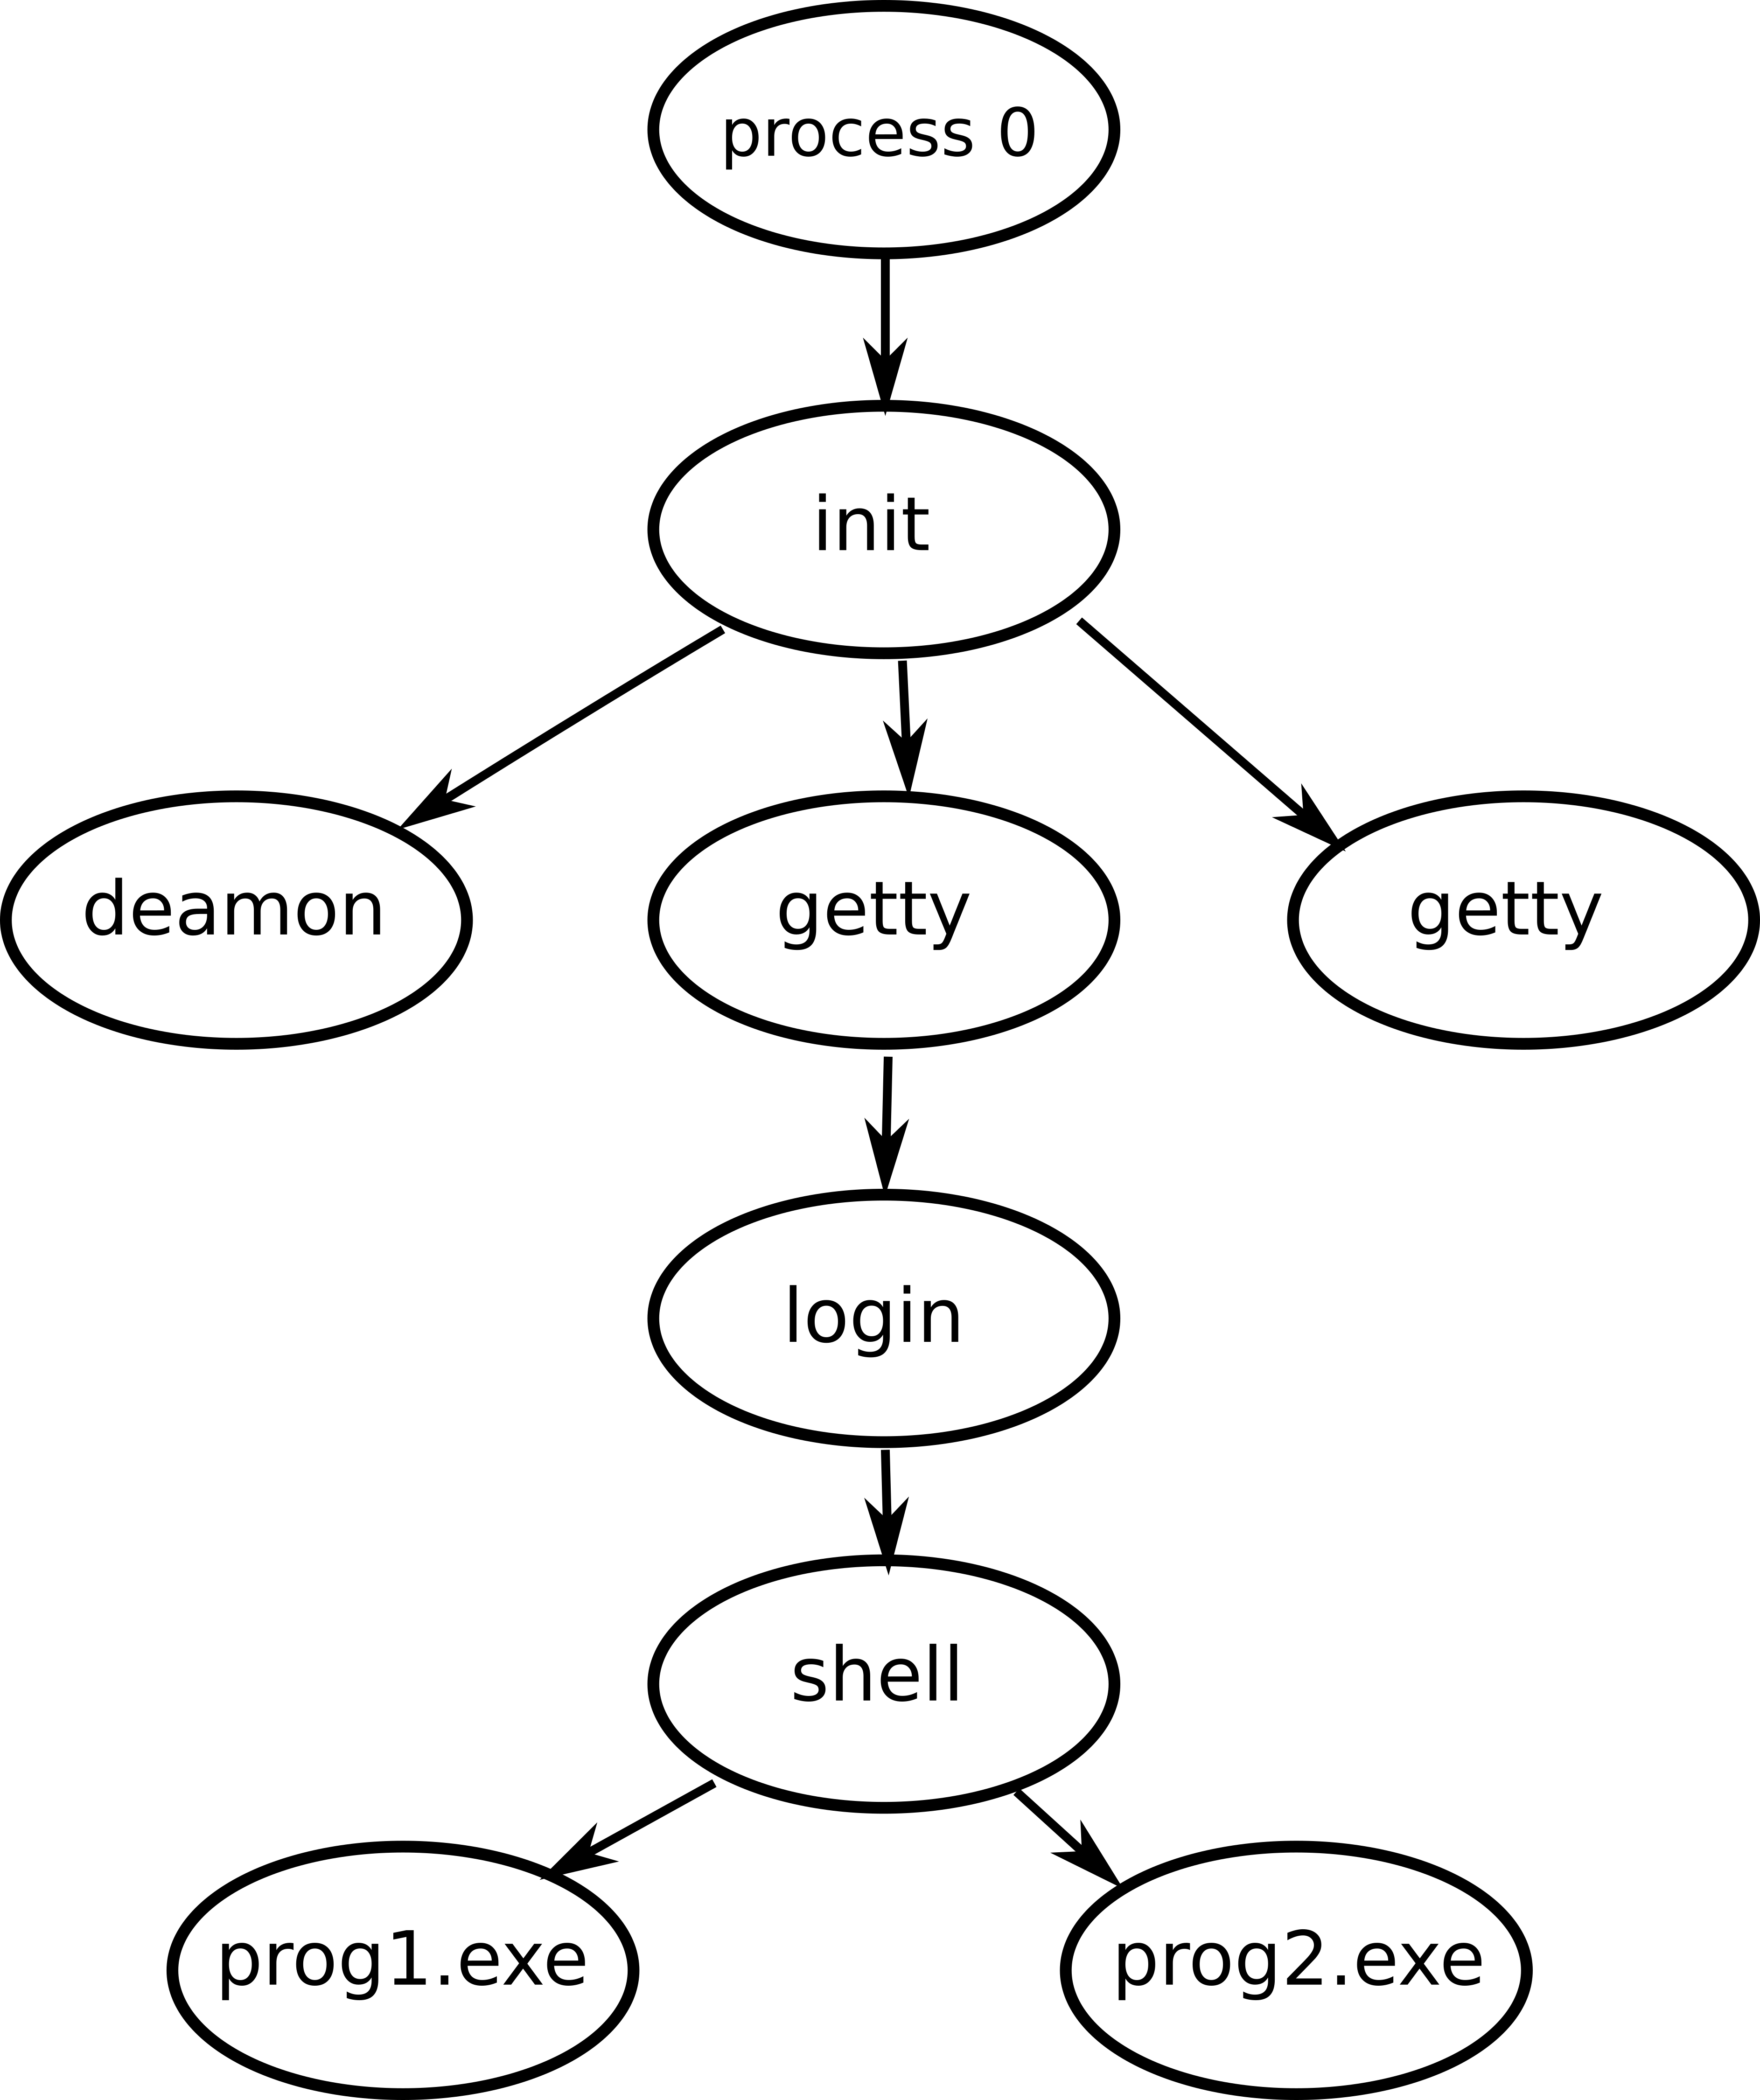
\includegraphics[scale=0.07]{images/unix_process.png} 
     	%\vspace*{-0.5em}
		%\caption{Floating gate transistor cell}
	\end{figure}
	
	\end{center}		
	
	
	\end{frame}	
	
	\begin{frame}
	
	With UNIX each process has an entry in a \textbf{table of processes}, with\footnotemark[3]:
	\vspace*{1em}
	\begin{itemize}
	\item{the pid of the process (process identifier)}
	\item{the state of the process}
	\item{scheduling information}
	\item{the state of the memory}
	\item{etc.}
	\end{itemize}		
	
	
	\footnotetext[3]{Basically these are the PCB information...}
	\end{frame}	
	
	\begin{frame}
	
	UNIX processes have \textit{three modes}:
	\vspace*{1em}
	\begin{itemize}
	\item{The \textbf{user mode}: classic execution mode for \textit{elected processes}}
	\item{The \textbf{kernel \textit{in memory} mode}: mode for \textit{elected processes} in \textit{supervision} mode, \textit{ready processes} or \textit{blocked processes}\footnotemark[4]}
	\item{The \textbf{swapped mode}: processes blocked for a too long time are placed into mass storage memory\footnotemark[5]}
	
	\end{itemize}

	\begin{center}
		
	\begin{figure}
		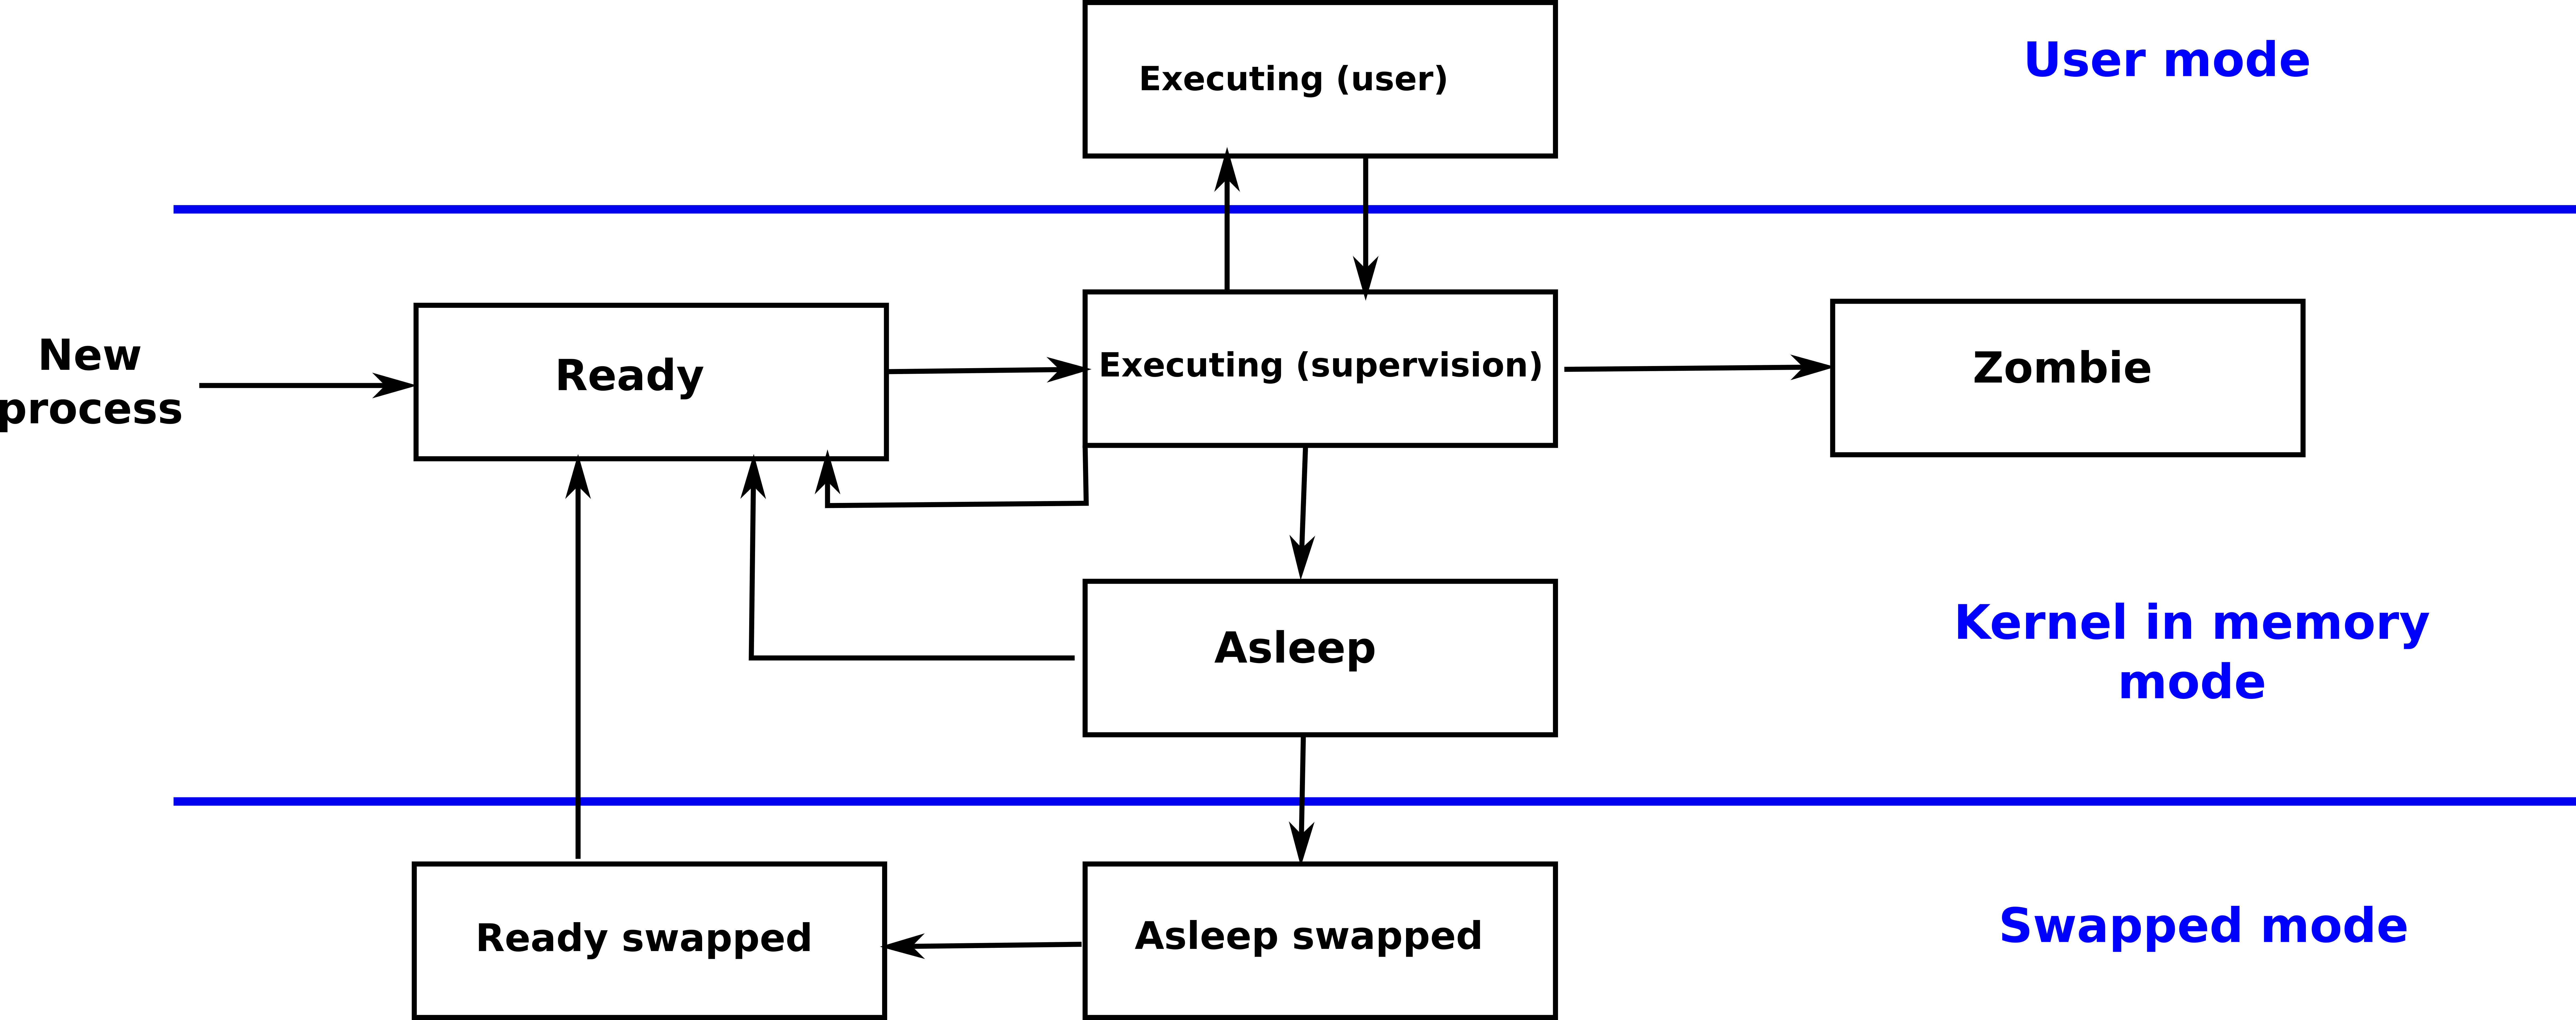
\includegraphics[scale=0.06]{images/unix_modes.png} 
     	%\vspace*{-0.5em}
		%\caption{Floating gate transistor cell}
	\end{figure}
	
	\end{center}	

	\footnotetext[4]{Terminated processes go into zombie state waiting for the PCB to be destroyed}
	\footnotetext[5]{When unblocked they join back the \textit{main memory}, and become \textit{ready}}
	
	\end{frame}
	
	\section{Scheduler}	
	\subsection{Introduction}	
	
	\begin{frame}
		
	\begin{block}{What does the scheduler?}	
	The \textit{scheduler} manages the \textbf{priority of execution} of the \textbf{processes} 
	\end{block}	
	\vspace*{1em}
	The \textit{scheduler} manages the \textbf{priority of execution} by
	\vspace*{1em}
	\begin{itemize}
	\item{...choosing which \textit{process} must be \textit{elected} first}
	\item{...choosing which \textit{processes} must be \textit{elected} after}
	
	\end{itemize}		
	
	\begin{center}
		
	\begin{figure}
		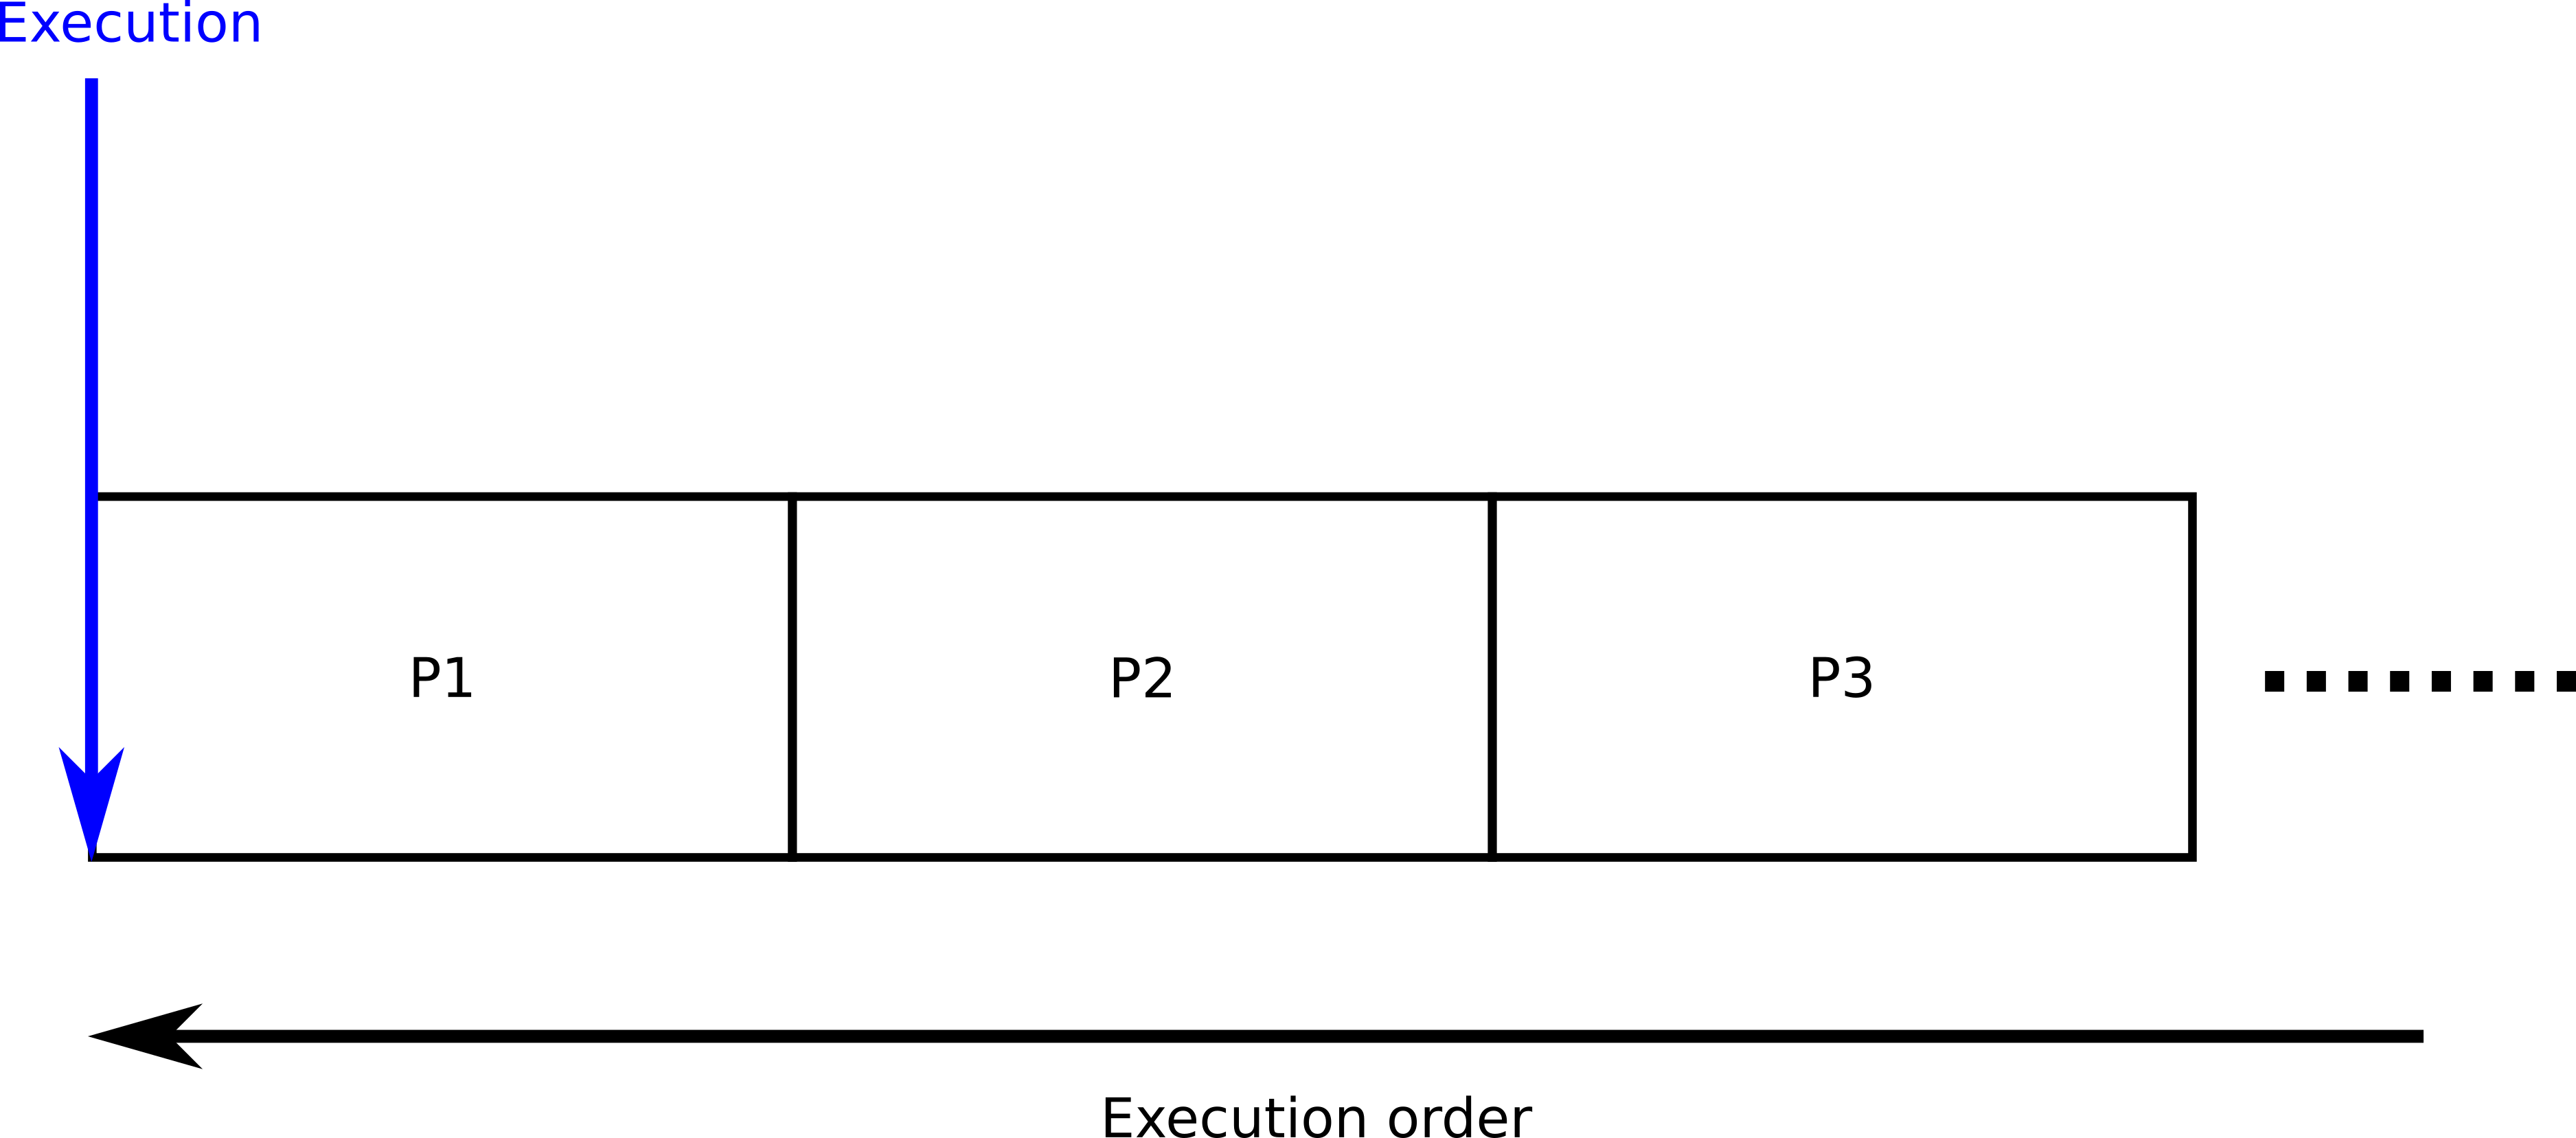
\includegraphics[scale=0.15]{images/process_execution.png} 
     	%\vspace*{-0.5em}
		%\caption{Floating gate transistor cell}
	\end{figure}
	
	\end{center}		
	
	
	\end{frame}
	
	\subsection{Scheduler and dispatcher}	
	
	\begin{frame}
	
	When dealing with one \textit{processor unit}, mo need of \textit{dispatcher}:
	\vspace*{1em}	
		\begin{figure}
		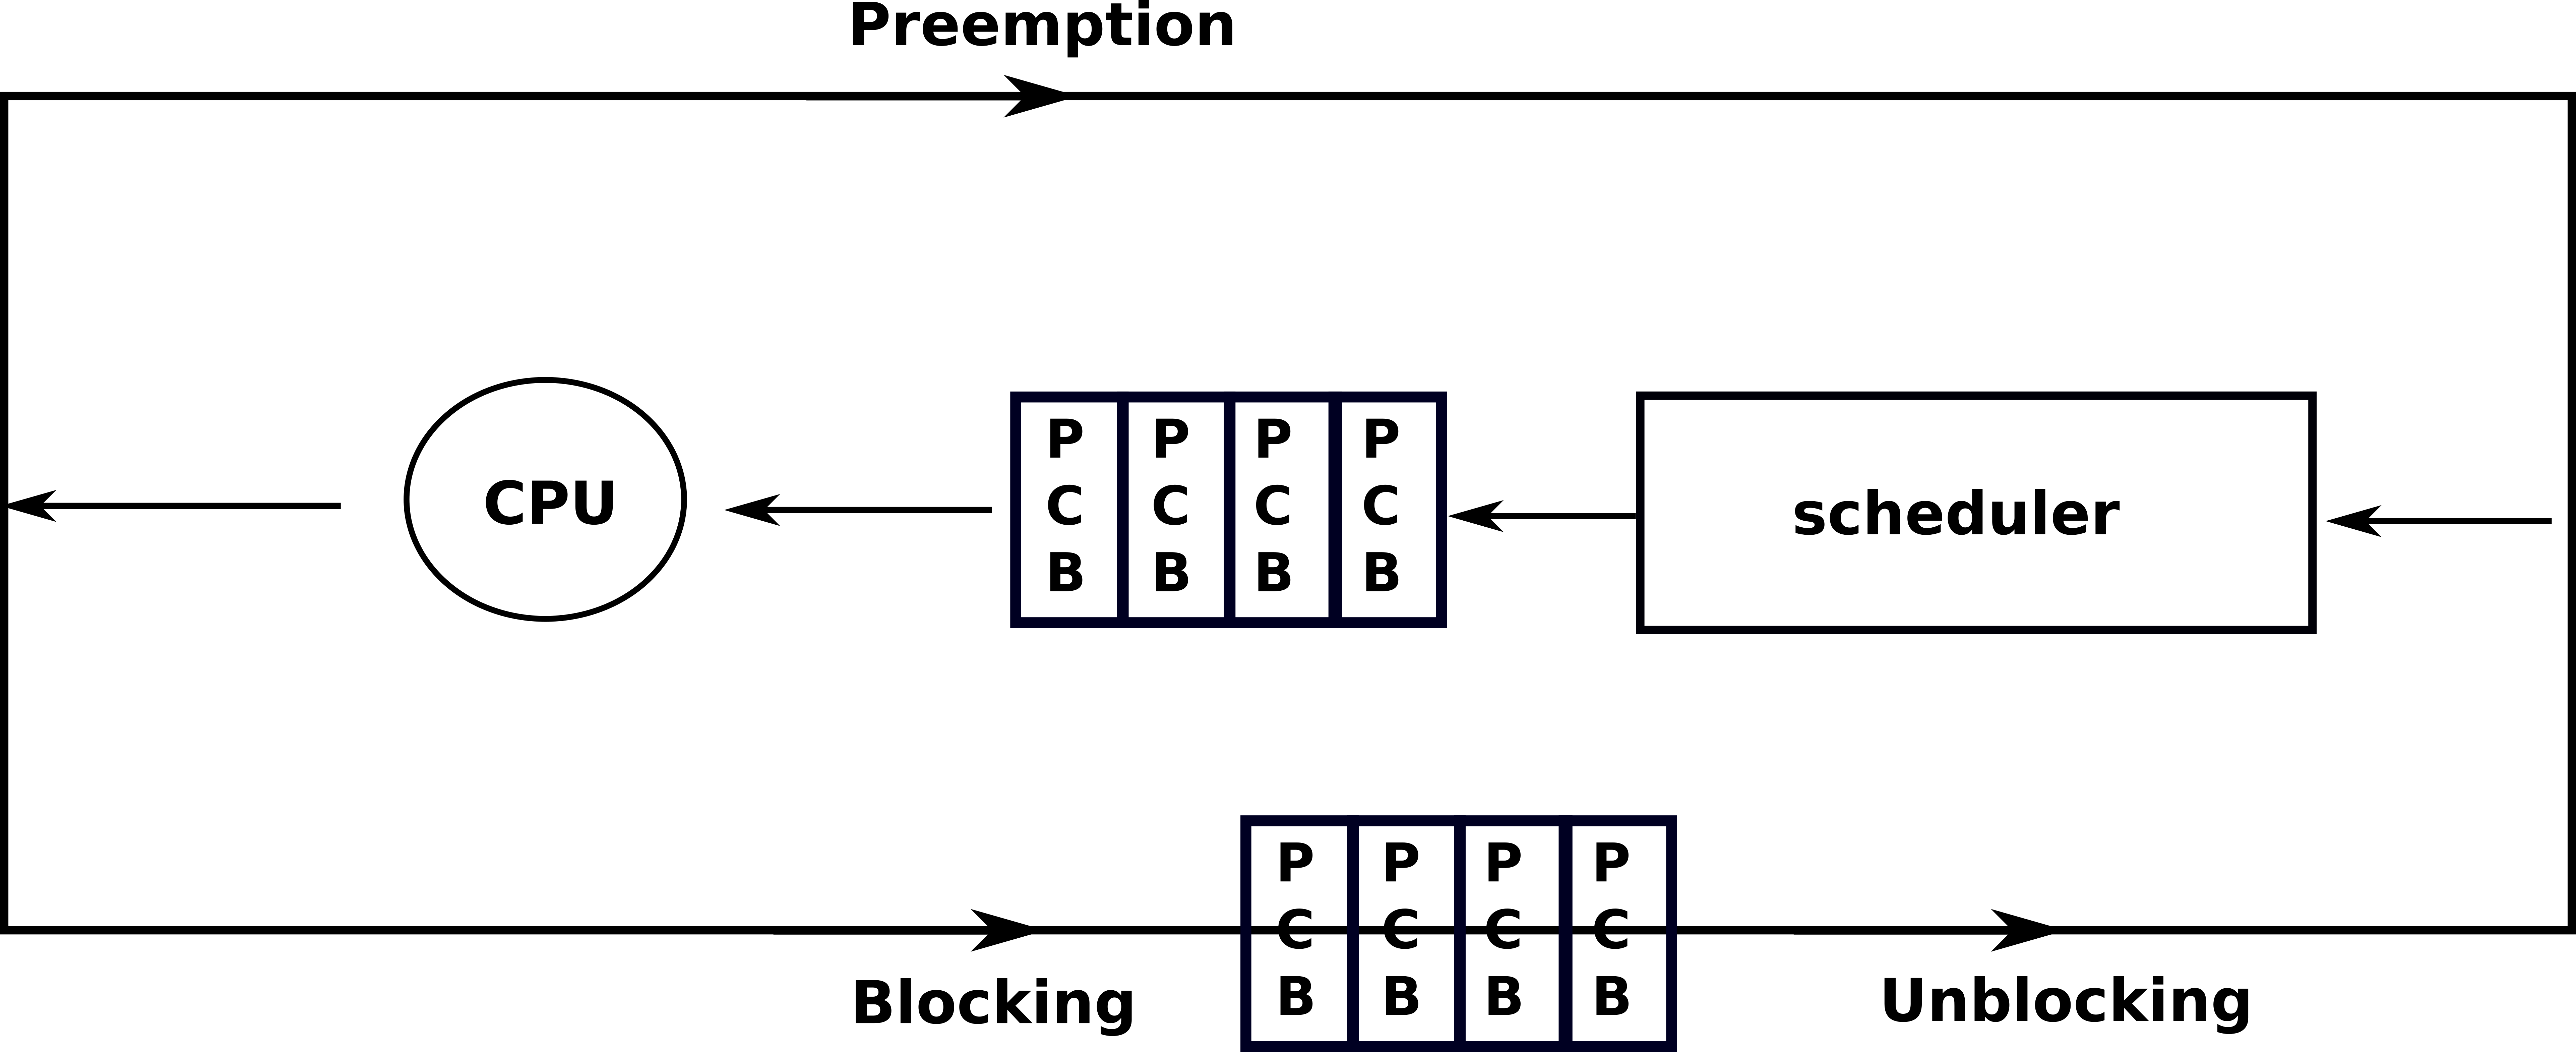
\includegraphics[scale=0.04]{images/dispatcher_1.png} 
     	%\vspace*{-0.5em}
		%\caption{Floating gate transistor cell}
	\end{figure}
	
	When dealing with several \textit{CPUs}, there is a \textit{dispatcher}:
		\vspace*{1em}	
		\begin{figure}
		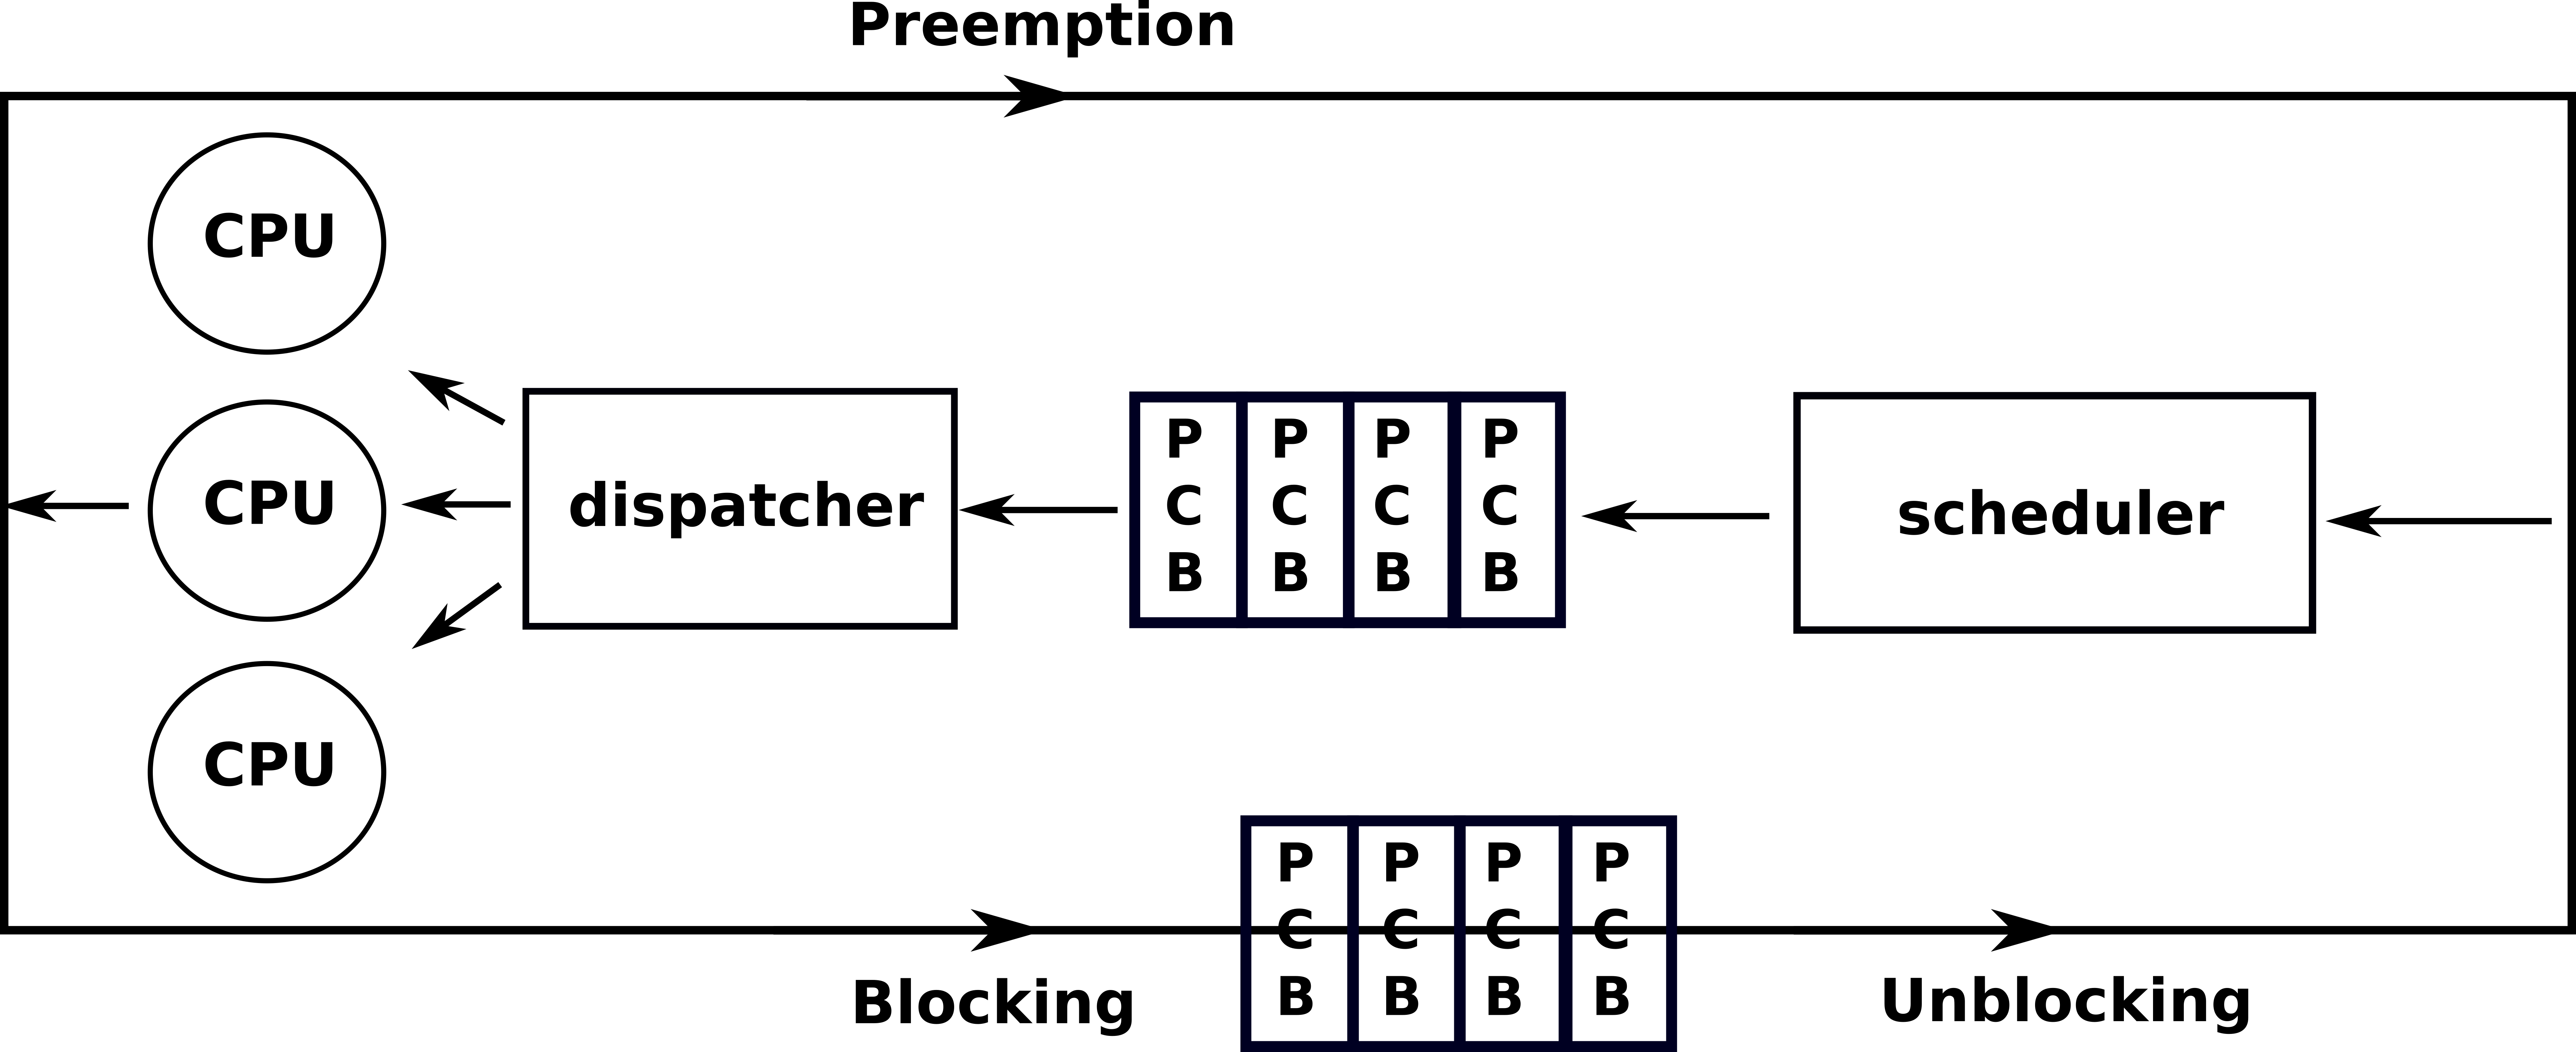
\includegraphics[scale=0.04]{images/dispatcher_2.png} 
     	%\vspace*{-0.5em}
		%\caption{Floating gate transistor cell}
	\end{figure}
	
	
	
	\begin{block}{Preemption}
	A \textit{preemption} is when the \textit{scheduler} \textbf{force a process to leave the CPU}	
	\end{block}	
		
			
		
		
	\end{frame}	
	
	\subsection{Scheduling policies}
	\begin{frame}
	
	\begin{block}{Policy?}
	The \textit{scheduler} \textbf{prioritize the order of execution} using a \textit{policy}:
	\begin{itemize}
	\item{The goal is to \textbf{optimize the overall time of execution}}
	\item{There are \textbf{different policies} for doing that}
	\end{itemize}		
	\end{block}	
		
	\vspace*{1em}
	Among the different possible \textit{policies} there are:
	\vspace*{1em} 
	\begin{itemize}
	\item{The \textbf{"First in, first executed"} \textit{policy}}
	\item{The \textbf{"Smallest time of execution first"} \textit{policy}}
	\item{The \textbf{"Biggest priority first"} \textit{policy}}
	\item{The \textbf{"Rate monotonic"} \textit{policy}}
	\item{The \textbf{"Round robin"} \textit{policy}}
	\end{itemize}
	
	\end{frame}
		
	\begin{frame}
	
	\begin{itemize}
	\item{The \textbf{"First in, first executed"} \textit{policy}:
		\begin{itemize}
		\item{\textit{Processes} executed in order of arrival}
		\item{Simple approach}
		\item{BUT: small \textit{processes} are penalized by big \textit{processes}}
		\end{itemize}
	}
	\vspace*{1em}
	\item{The \textbf{"Smallest time of execution first"} \textit{policy}:
		\begin{itemize}
		\item{Smallest \textit{processes} are executed first}
		\item{Here it's the minimal average of time of answer!}
		\item{BUT: you need to know how much time last the \textit{processes}}
		\end{itemize}	
	}
	\vspace*{1em}
	\item{The \textbf{"Biggest priority first"} \textit{policy}:
	\begin{itemize}
	\item{Each process has a priority number: highest priorities are first}
	\item{BUT: processes with low priorities may be executed very late!}
	\end{itemize}
	
	
	
	}
	\end{itemize}		
	
	
	\end{frame}			
		
	\begin{frame}
	
	\begin{itemize}
	\item{The \textbf{"Rate monotonic"} \textit{policy}:
		\begin{itemize}
		\item{Each \textit{process} has a priority number}
		\item{The priority number is proportionate to the frequency of the \textit{process}}
		\item{\textit{Processes} needing to be launched frequently are in top priority}
		\item{Once ready again, a high frequency \textit{process} will be elected in priority}
		\end{itemize}
	}
	\vspace*{1em}
	\item{The \textbf{"Round robin"} \textit{policy}:
	\begin{itemize}
	\item{Each \textit{process} is executed in a specific amount of time (10ms to 100ms)}
	\item{If it lasts more: the \textit{process} is preempted until elected again}
	\item{The whole context is stored in the \textit{PCB} to resume after}
	\item{Preempted \textit{processes} are resumed later using a queue:}
	\end{itemize}
		\vspace*{1em}	
		\begin{figure}
		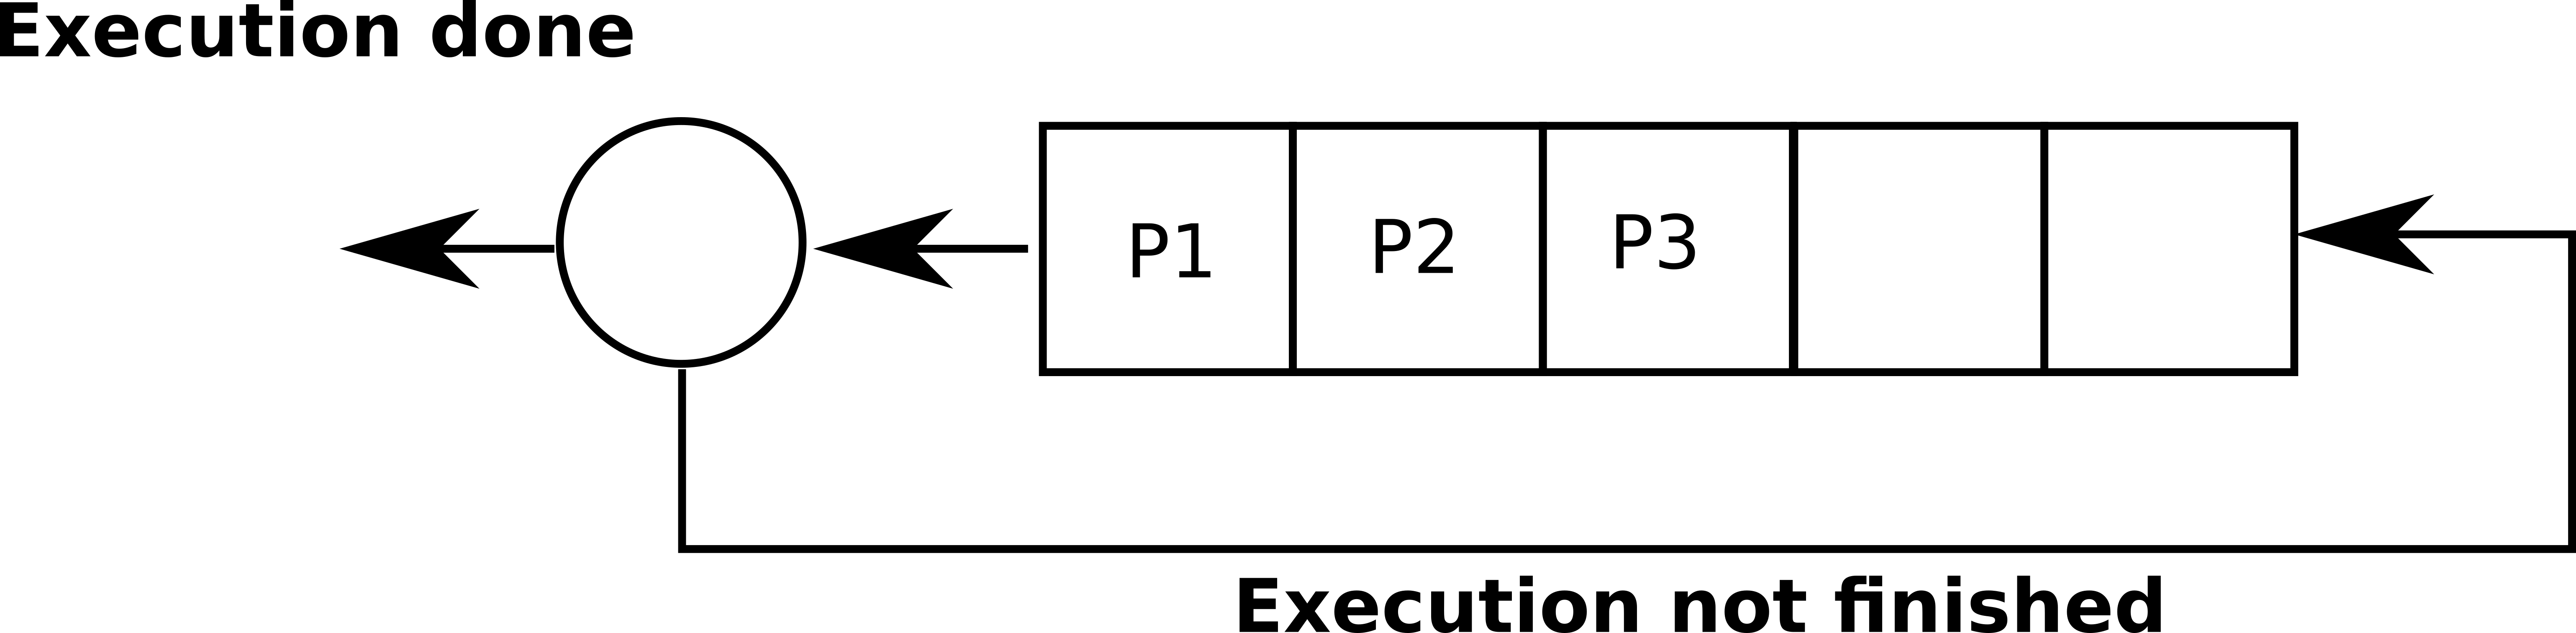
\includegraphics[scale=0.09]{images/robin.png} 
     	%\vspace*{-0.5em}
		%\caption{Floating gate transistor cell}
	\end{figure}
	
	}
	\end{itemize}
	
	\end{frame}		
	
	\subsection{Linux scheduler}	
	
	\begin{frame}	
	
	With Linux:
	\vspace*{1em}
	\begin{itemize}
	\item{Each \textit{process} has a priority number}
	\item{There are three different scheduling \textit{policies}:
		\begin{itemize}
		\item{\textbf{SCHED\_FIFO}: elect processes with the highest priorities 
			\begin{itemize}
			\item{for the most important processes}
			\end{itemize}
		}
		\item{\textbf{SCHED\_RR}: robin round policy between processes 
			\begin{itemize}
			\item{for processes with same priority number!}
			\item{for the most important processes}
			\end{itemize}	
		}					
		\item{\textbf{SCHED\_OTHER}: elect processes with the highest priorities
			\begin{itemize}
			\item{for all classes!}
			\end{itemize}				
		}
		\end{itemize}			
	}
	\end{itemize}

	\begin{block}{Note}
	\begin{itemize}
	\item{Processes attached to SCHED\_FIFO and SCHED\_RR are more important}
	\item{SCHED\_OTHER execute the remaining processes}
	\end{itemize}
	\end{block}
	
	\end{frame}
	
\end{document}
